%%% Thesis Introduction --------------------------------------------------
\chapter*{Introduction}
\fancyhead{}
\fancyhead{}
% \ifpdf
%     \graphicspath{{Introduction/IntroductionFigs/PNG/}{Introduction/IntroductionFigs/PDF/}{Introduction/IntroductionFigs/}}
% \else
%     \graphicspath{{Introduction/IntroductionFigs/EPS/}{Introduction/IntroductionFigs/}}
% \fi

%\pagestyle{empty}

%\thispagestyle{plain}
\renewcommand{\LettrineFontHook}{\color{red}}


\lettrine[lines = 3, loversize=-0.1, lraise=0.1]{F}{}rom the dawn of
its existence astronomy has always been starving for data but in the
last few decades the situation has changed and now we are facing data
deluge of biblical proportions. The data are not just increasing in
size but also in complexity and dimensionality
\citep{ballastroinformatics}. Astroinformatics is the new field of
science which has emerged from this technology driven progress.
Virtual Observatory, Machine Learning, Data Mining, Grid Computing are
just few examples of new tools available to scientists.


\vspace{10pt}
\begin{figure}[!htbp]
  \begin{center}
    \leavevmode
    \ifpdf
    \includegraphics[scale = .8]{astroinformatics}
    \else
    \includegraphics[bb = 92 86 545 742, height=6in]{astroinformatics.png}
    \fi
    \caption{Astroinformatics in the context of astronomy \citep{ballastroinformatics} }
    \label{FigAir}
  \end{center}
\end{figure}
\vspace{-10pt}



The astronomers are not alone and particle physics, biology and other
sciences are also in the vanguard of the data intensive science. This
is great opportunity for interdisciplinary collaboration.

This work deals with the problem of semi-automatic procedures for
finding Be stars \citep{porter2003classical} candidates in the
astronomy surveys. More than straight forward process it's trail and
error approach probing new possibilities with rather interesting than
useful results.

The aim of this work is to be introductory to the technologies of
Virtual Observatory and massive data processing in general.

%  and for this reason it is intended
% to have following properties:

% \begin{itemize}
% \item Main Chapters starts with diagram to ease orietation,
% \item is full of examples, 
% \item is non-linear in nature,
% \item is meant to be compact and consistent,
% \item is far from complete.
% \end{itemize}

\begin{figure}[!htbp]
  \begin{center}
    \leavevmode
    \ifpdf
    \includegraphics[scale = 1]{mapThesis}
    \else
    \includegraphics[bb = 92 86 545 742, height=6in]{mapThesis}
    \fi
    \caption{Thesis structure}
    \label{FigStructure}
  \end{center}
\end{figure}


Chapter one is an introduction to the technologies related to Virtual
Observatory. The motivation behind the concept is given without paying
too much attention to historical details. Main principles and
protocols are discussed and explained. Important aspect are
demonstrated on numerous examples. Chapter two is an introduction to
Machine Learning and Data Mining in the context of astrophysics. Only
methods used in practical part of this work are described in detail:
Decision Trees and Support Vector Machines. Examples of several
classifications are demonstrated. Third chapter introduces issues of
Be stars. Chapter Four is practical application of previously
described technologies and methods. Training data of confirmed Be
stars from Ondrejov are correlated with others catalogues to obtain
color indexes and spectra. Results are processed by Data Mining
algorithms using several libraries and tools. In the last chapter
achieved results are critically discussed.

Many scripts were written to achive individual goals. In the text
there are numerous commented snippets of codes. Their purpose is to
demonstrate the concept and they are thefore short and without
auxiliary technicalities such are error handling etc. They are mostly
Python and shell scripts. Any interested person can obtain the full
source codes (including thesis itself) from GIT repository
\footnote{\url{git://github.com/astar/diplomaWork}}.


\begin{table}[ht]
  \centering
  \small
     \begin{tabular}[ht]{l l}
     \toprule
     Name & Description \\
     \midrule
     analyse & Check the wavelength range, raname according to
     target name\\
     getSpectraList & Create SSA Compliant list from\\
     getSpectra & Get spectra links from SSA Server\\
     madmax & Extract feautres from spectra \\
     convolve &  Reduction of Ondřejov's spectra\\
     pf & Print Fits. Shows the spectrum \\
     dm &  Perform classification\\
     makeHTML & Creates HTML pages of results \\ 
     \bottomrule
   \end{tabular}
  \caption{Scripts developed within the scope of the thesis.}
  \label{tab:scripts}
\end{table}


Activities related to this work went beyond this text. Wiki
pages\footnote{\url{http://physics.muni.cz/~vazny/wiki/index.php/Diploma_work}}
were created to present the results and discuss related topic with
supervisor as well as with others scientist around the world. Source
codes were maintained by GIT version system allowing easy sharing. All
software used and produced are open source.





%%% ----------------------------------------------------------------------


%%% Local Variables: 
%%% mode: latex
%%% TeX-master: "../thesis"
%%% End: 
